\chapter{Experimental Facts}
\label{chap0}
\begin{enumerate}
	\item (6) Show that every galilean transformation of the space $ \R\times\R^3$ can be written in a unique way as the composition of a rotation, a translation, and a uniform motion ($ g = g_1 \circ g_2 \circ g_3 $)(thus the dimension of the galilean group is equal to $3+4+3 = 10$).\par
	
	Solution: We first consider a general linear transformation on $ \R\times\R^3$ as the $ 4\times 4 $ matrix $ A $ and an affine transformation $G$ given by $G a = A a+\lambda$ for any $a\in \R\times\R^3$ where $\lambda$ is a constant vector. Since we require $A$ to preserve the galilean structure, $G$ has to preserve the time interval between two events $t(b-a)$, as well as the distance between two simultaneous events $\rho (a, a') = ||a-a'||$. To summarize, $ G $ has to satisfy
	\begin{align}
		t(a-b) &= t(Ga-Gb)\\
		\rho(a,a') &= \rho(Ga, Ga').
	\end{align} 
	We now explicitly write out the transformation of an event $a\in \R\times \R^3$ under $G$.
	\begin{equation}
		Ga = \begin{pmatrix}
			A_{00} & A_{01} & A_{02} & A_{03}\\
			A_{10} & A_{11} & A_{12} & A_{13}\\
			A_{20} & A_{21} & A_{22} & A_{23}\\
			A_{30} & A_{31} & A_{32} & A_{33}
		\end{pmatrix}\begin{pmatrix}
		a^0\\ a^1\\ a^2\\ a^3 
	\end{pmatrix}+\begin{pmatrix}
	\lambda^0\\\lambda^1\\ \lambda^2\\\lambda^3
\end{pmatrix}
		= \begin{pmatrix}
			A_{0i}a^i+\lambda_0\\ A_{1i}a^i+\lambda^1 \\ A_{2i}a^i+\lambda^2\\A_{3i}a^i+\lambda^3
	\end{pmatrix}
	\end{equation}
where repeated indices are summed over $i = 0,..3$. The difference in the coordinate $i = 0$ is taken as the time interval map for $\R \times \R^3$, i.e., $t(a-b) = a^0-b^0$. For the invariance of the time interval between two events $a$ and $b$, we have
\begin{equation}
a^0-b^0 = A_{00}(a^0-b^0) + A_{01}(a^1-b^1)+...
\end{equation}
Since this has to hold for any two events, we are led to the conclusion that $A_{00} = 1$ and $A_{0i} = 0$, $ i = 1,2,3$. Now to preserve distances for two simultaneous events $a$ and $a'$ ($a^0 = a'^0$),
\begin{equation}\label{key}
	\sum_{i,j=1}^3 (A_{ij}(a^j-a'^j))^2 = 	\sum_{i=1}^3 (a^i-a'^i)^2
\end{equation}
Thus the cofactor matrix $A^C = [A^C_{00}]$ obtained by removing the first row and first column must be an orthogonal matrix ($(A^{C})^{\mathrm{T}}A^C = I_3 $, where $I_3$ is the $3\times3$ identity matrix). Thus, a distance and time interval preserving transformation on $\R\times \R^3$ can be written down as 
\begin{equation}\label{genA}
	A = \begin{pmatrix}
		1 & 0 & 0 & 0\\
		v_1&R_{11}& R_{12}& R_{13}\\
		v_2&R_{21}&R_{22} &R_{23} \\
		v_3&R_{31}& R_{31}& R_{33}
		\end{pmatrix}
\end{equation}
where $R_{i,j}$ are the elements of a $3\times 3$ orthogonal matrix $R$, and $v_1, v_2, v_3$ represent the elements $A_{10}, A_{20}, A_{30}$ of $A$ respectively. To see that these terms represent a boost, we consider the action of a transformation $ A_{\mathrm{boost}} $ with $R=I_3$
\begin{equation}\label{key}
	A_{\mathrm{boost}} a = \begin{pmatrix}
			a^0\\
			v_1 a^0 + a^1\\
			v_2 a^0 + a^2\\
			v_3 a^0 + a^3	
		\end{pmatrix}
\end{equation}
which represents the original point moving with a speed given by $\mathbf{v} = (v_1, v_2, v_3)$. Thus, we see that the final galilean transformation can be written down as 
\begin{equation}
	G a  = A_\mathrm{boost}A_\mathrm{orthogonal} a + \lambda
\end{equation}
with \begin{equation}\label{key}
	 A_{\mathrm{boost}} = \begin{pmatrix}
	 	1 & 0 & 0 & 0\\
	 	v_1&1& 0& 0\\
	 	v_2&0&1 &0 \\
	 	v_3&0& 0& 1
	 \end{pmatrix}\hspace{1cm} A_{\mathrm{orthogonal}} = \begin{pmatrix}
	 1 & 0 & 0 & 0\\
	 0&R_{11}& R_{12}& R_{13}\\
	 0&R_{21}&R_{22} &R_{23} \\
	 0&R_{31}& R_{31}& R_{33}
 \end{pmatrix}
\end{equation}
where the boost and rotation operations commute and can be well defined by the combined matrix $A$ from \eqref{genA}.\qed
\item (6) Show that all galilean spaces are isomorphic to each other and, in particular, isomorphic to the coordinate space $\R\times\R^3$.\par
Solution: Let $E, E'$ be galilean spaces with underlying vector space $\R^4$ , i.e., for any $a,b\in E$ or $E'$, $a-b\in \R^4$. If we can find isomorphisms $\phi:E\rightarrow \R\times\R^3$ and $\phi':E'\rightarrow \R\times\R^3$, then we can construct the isomorphism $\phi'^{-1}\circ\phi:E\rightarrow E'$ which is the required isomorphism between two arbitrary galilean spaces.\par
We first construct a map $M:\R^4\rightarrow\R\times\R^3$ that maps the time coordinate to the 0 index (thus the notation $\R\times \R^3$). The time map is a linear map $T:\R^4\rightarrow\R$. Let $e_0,...e_3$ be an arbitrary basis for $\R^4$. Then 
\begin{align}
	v &= v^ie_i\\
	Tv & = v^i (Te_i)
\end{align}
We want to construct a basis $e'_i$ where $T(e'_i) = \delta_{0i}$. Let the required transformation matrix be $M$, $ e'_i = (M^{-1})_i^{j}e_j $. To satisfy the condition, $(M^{-1})_i^{j} T(e_j) = \delta_{0i}\implies T(e_j) = M^i_j\delta_{0i} = M^0_j$. For the remaining indices, we are free to choose any $3\times 4$ matrix such that $M$ is full-rank. Not all $T(e_i)$ can be zero, so assume that at least $T(e_3)$ is non-zero. We set
\begin{equation}\label{key}
	M = \begin{pmatrix}
		T(e_0)&T(e_1)&T(e_2)&T(e_3)	\\
		1 &0 & 0&0\\
		0&1&0&0\\
		0&0&1&0
	\end{pmatrix}.
\end{equation}
 Note that this choice is unimportant as even if all but one of the terms $T(e_i)$ with $i\neq 3$ is zero, we can set the cofactor matrix $[M^C_{0i}]$ to $I_3$ so that $M$ thus defined is full rank. Now,
\begin{align}
	v'^ie'_i &= v^k e_k\\
	v'^i(M^{-1})_i^{j}e_j &= v^k e_k\\
	\implies v'^i (M^{-1})_i^{j} &= v^j\\
	\implies v'^i &= M^i_j v^j
\end{align}
Thus, we have a map $M: \R^4 \rightarrow \R\times\R^3$ such that $Tv = (Mv)^0$ i.e., we have separated the time coordinate $\R$ from the spacial coordinates $\R^3$ of $v$. Since $M$ is full-rank, the map is also invertible. \par
Now let $c\in E$ be fixed. Then we can write any $a\in E$ in the form $a = c + v$ where $v\in \R^4$ (this is effectively choosing an origin), define the map $P_c: E\rightarrow \R^4$ such that $ P_c(a) = a-c = v\in \R^4 $, which is clearly invertible ($P_c^{-1}(v)  = c+v$). Now construct the composite map $\phi_c = M\circ P_c : E\rightarrow\R\times\R^3$. This is the required isomorphism. Note that this is not a canonical isomoprhism as one can make any choice for the "origin" $c\in E$. \qed

\begin{figure}
	\centering
	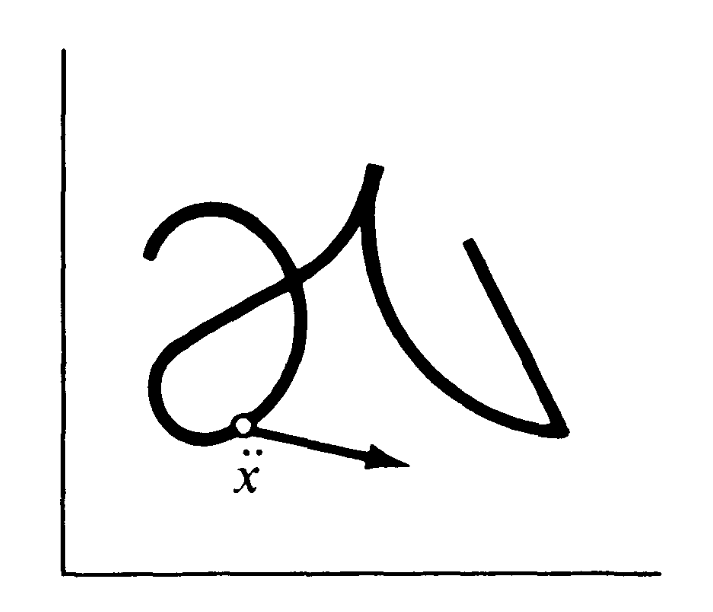
\includegraphics[width=0.5\linewidth]{7}
	\caption[Trajectory of motion of a particle]{}
	\label{fig:7}
\end{figure}

\item (7) Is it possible for the trajectory of a differentiable motion on the plane to have the shape drawn in Figure \ref{fig:7}? Is it possible for the acceleration
vector to have the value shown?\par
Solution: The trajectory shown is a perfectly reasonable motion. However, the acceleration vector shown is not possible. The velocity vector at every point on the curve points in the direction of the tangent to the curve.
The direction of change of the tangent vector is given by the acceleration vector. Clearly, the tangent vector changes "inward" rather than "outward" as indicated by the arrow.
\item (10) Show that if a mechanical system consists of only one point, then
its acceleration in an inertial coordinate system is equal to zero ("Newton's
first law").\par
Solution: If there is only one point  in the system, $\ddot{\mathbf{x}} = \mathbf{f}(t, \mathbf{x},\dot{\mathbf{x}})$ is invariant under translations in time or space and under boosts with constant velocity. This implies \begin{align}\label{key}
	\mathbf{f}(t, \mathbf{x},\dot{\mathbf{x}}) &= \mathbf{f}(t+s, \mathbf{x},\dot{\mathbf{x}})&&\implies  \mathbf{f} = \mathbf{f}(\mathbf{x},\dot{\mathbf{x}}))\\
	\mathbf{f}(\mathbf{x},\dot{\mathbf{x}}))& = 	\mathbf{f}(\mathbf{x}+\mathbf{x_0},\dot{\mathbf{x}}))&&\implies  \mathbf{f} = \mathbf{f}(\dot{\mathbf{x}})\\
	\mathbf{f}(\dot{\mathbf{x}})& = \mathbf{f}(\dot{\mathbf{x}}+\mathbf{v_0}) &&\implies \mathbf{f} = const.
\end{align}
Invariance under orthogonal translations thus implies that $ \mathbf{f} = 0 $.\qed
\item (10) A mechanical system consists of two points. At the initial moment
their velocities (in some inertial coordinate system) are equal to zero. Show
that the points will stay on the line which connected them at the initial
moment.\par
Solution: Let the point be 1 and 2. Choose a coordinate system such that at $t = 0$, $\mathbf{x}_1(0) = a \mathbf{u}_0$, $\mathbf{x}_2(0) = b \mathbf{u}_0$, and $\mathbf{\dot{x}}_1(0) = \mathbf{\dot{x}}_2(0)=0$, where $a$ and $b$ are constants and $u_0$ is a vector parallel to the line joining 1 and 2. The forces on 1 and 2 are given by $\mathbf{f_i}(\mathbf{x_1}-\mathbf{x_2}, \mathbf{\dot{x}}_1-\mathbf{\dot{x}}_2.)$\par
Now, we note that if $\mathbf{v}, \mathbf{w} \in \R^3$ are such that $\mathbf{v} = c \mathbf{w}$ for some $c\in \R$, a rotation $R$ about the $\mathbf{v}$ leaves both vectors unchanged, i.e., $R\mathbf{v} = \mathbf{v}$, $ R\mathbf{w} = \mathbf{w} $ . Then 
\begin{align}
	\mathbf{f}_i(R\mathbf{v},R\mathbf{w}) &= R\mathbf{f}_i(\mathbf{v},\mathbf{w})\\=\mathbf{f}_i(\mathbf{v},\mathbf{w})&\\
	R\mathbf{f}_i(\mathbf{v},\mathbf{w}) = \mathbf{f}_i(\mathbf{v},\mathbf{w})
\end{align}
Thus, if at any point the displacement and relative velocities are parallel to some vector $\mathbf{v}$, the force acting on the particles are also parallel to $\mathbf{v}$.\par
Back to our problem, define the function $F_i(x,y) \mathbf{u_0} \equiv \mathbf{f}_i(x\mathbf{u_0},y\mathbf{u_0})$. Let $y_i(t)$ be the solution to the system $\ddot{y_i} = F_i(y_1-y_2, \dot{y_1}-\dot{y_2})$, with initial conditions $y_1(0) = a$, $y_2(0) = b$, and $\dot{y_1}(0) = \dot{y_2}(0) = 0$. We can show that $\mathbf{x}_i(t) = \mathbf{u_0}y_i(t)$ is a solution to the original problem and thus the points always remain on the line parallel to $u_0$.
\begin{align}
	\ddot{\mathbf{x}}_i& = \mathbf{u_0}\ddot{y}_i\\
	& =\mathbf{u_0} F_i(y_1-y_2, \dot{y_1}-\dot{y_2})\\
	& = \mathbf{f}_i(\mathbf{u_0}(y_1-y_2), \mathbf{u_0}(\dot{y_1}-\dot{y_2})\\
	&=\mathbf{f}_i(\mathbf{x_1}-\mathbf{x_2},\dot{\mathbf{x}}_1-\dot{\mathbf{x}}_2)
\end{align}
This solution is unique since the solution for the $y_i$'s are unique. \qed
\item (10) A mechanical system consists of three points. At the initial moment
their velocities (in some inertial coordinate system) are equal to zero.
Show that the points always remain in the plane which contained them at the
initial moment.\par
Solution: Let the three points be 1, 2, 3. At $t =0$, they lie on some plane $\tau$ with normal $\mathbf{N}$, and we are free to choose inertial coordinates that set the origin as $\mathbf{x}_1(0)$. Then $\mathbf{x}_2(0)-\mathbf{x}_1(0) = \mathbf{u}_0$, $\mathbf{x}_3(0)-\mathbf{x}_1(0) = \mathbf{v}_0$ are vectors that lie on $\tau$ and are perpendicular to $\mathbf{N}$.\par

We now note that reflections are also distance preserving transformations and are also a valid galiliean transformations\footnote{Reflections are discrete transformations as opposed to the continuous translation, boost and rotation. The set of all galilean transformations barring rotations forms a Lie Group (see \ref{chap8}).} (this is a problem in this chapter which we will argue now to proceed with this problem). Reflections are orthogonal transformations with $\mathrm{det}G = -1$. Invariance  with respect to reflections means that there are no preferred orientations of coordinates in space. Thus we have the relation 
\begin{equation}
	\mathbf{F}(G\mathbf{x},G\dot{\mathbf{x}}) = G \mathbf{F}(\mathbf{x},\dot{\mathbf{x}})
\end{equation}

The forces that enter the equations of motion are functions of $\mathbf{x_i}-\mathbf{x_j}$ and $\dot{\mathbf{x_i}}-\dot{\mathbf{x_j}}$ , i.e., $ \mathbf{f}_i  = \mathbf{f}_i(\mathbf{x_2}-\mathbf{x_1},\mathbf{x_3}-\mathbf{x_1},\dot{\mathbf{x_2}}-\dot{\mathbf{x_1}},\dot{\mathbf{x_3}}-\dot{\mathbf{x_1}})$. Let $\mathbf{w_1}, \mathbf{w_2}, \mathbf{w_3}, \mathbf{w_4}\in \textit{Span}(\mathbf{u_0}, \mathbf{v}_0)$, and G denote the reflection through the direction $\mathbf{N}$. Clearly, $G\mathbf{u}_0 = \mathbf{u}_0$ and $G\mathbf{v}_0 = \mathbf{v}_0$ and thus similar relations hold for the $\mathbf{w}_i$. Let $\mathbf{f}_i(\mathbf{w_1}, \mathbf{w_2}, \mathbf{w_3}, \mathbf{w_4}) = \mathbf{f}_{i}^{||}+ \mathbf{f}_{i}^{\perp}$ denote the components parallel and perpendicular to the plane $\tau$ (or perpendicular and parallel the normal $\mathbf{N}$) respectively. Now
\begin{equation}\label{incons1}
	G \mathbf{f}_i = G\mathbf{f}_{i}^{||} + G \mathbf{f}_{i}^{\perp} = \mathbf{f}_{i}^{||} -  \mathbf{f}_{i}^{\perp}.
\end{equation}
But from galilean invariance we have
\begin{equation}\label{incons2}
	G \mathbf{f}_i(\mathbf{w}_1,...) = \mathbf{f}_i(G\mathbf{w}_1,...) = \mathbf{f}_i(\mathbf{w}_1,...) = \mathbf{f}_{i}^{||}+ \mathbf{f}_{i}^{\perp}
\end{equation}
Equations \eqref{incons1} and \eqref{incons2} imply that $ \mathbf{f}_{i}^{\perp} = 0$. Thus if all arguments $\mathbf{w}_i$ lie on a plane, the forces $\mathbf{f}_i$ on all the particles also lies on the same plane.  \par

Now we define \begin{multline}\label{key}
	\mathbf{f}_i(a_1\mathbf{u_0}+b_1\mathbf{v_0}, ...,a_4\mathbf{u_0}+b_4\mathbf{v_0})\equiv\\ \mathbf{u_0}F_i^0(a_1, b_1,...a_4,b_4)+\mathbf{v_0}F_i^1(a_1,b_1,...,a_4,b_4)
\end{multline}
Let $y_i^j(t)$ be the solutions for $\ddot{y}_i^j = F_i^j(y_2^j-y_1^j, y_3^j-y_1^j ,\dot{y}_2^j -\dot{y}_1^j, \dot{y}_3^j-\dot{y}_2^j)$, with initial conditions $y_1^0(0) = y_1^1(0) = 0$, $y_2^0(0) = 1, y_2^1(0) = 0$, $y_3^0(0) = 0, y_3^1(0) = 1$ and $\dot{y}_i^j(0) = 0$ for $i = 1,2,3$ and $j = 1,2$.  Consider solutions of the form $ 	\mathbf{x}_i(t) = y_i^0(t) \mathbf{u}_0 + y_i^1(t) \mathbf{v}_0 $. Similar to the previous problem, it can be shown that these are also valid solutions. Now the system of differential equations for the $y_i^j$ are 6 second order equations with 12 initial conditions and thus possess a unique solution and thus, this solution for the $\mathbf{x}_i$ are unique. Thus we have shown that the trajectories of three particles stay on a plane if they started from rest in some inertial coordinate.\qed
\item (10) A mechanical system consists of two points. Show that for any
initial conditions there exists an inertial coordinate system in which the
two points remain in a fixed plane.\par
Solution: Let the two points be 1 and 2. They have initial conditions $\mathbf{x}_1(0) = \mathbf{a}_1$, $\mathbf{x}_2(0) = \mathbf{a}_2$, $\dot{\mathbf{x}}_1(0) = \mathbf{u}_0$, and $\dot{\mathbf{x}}_2(0) = \mathbf{v}_0$. The equations of motion take the form\begin{equation}\label{key}
	\ddot{\mathbf{x}}_i = \mathbf{f}_i(\mathbf{x}_1-\mathbf{x}_2, \dot{\mathbf{x}}_1-\dot{\mathbf{x}}_2)
\end{equation}
Let $\mathbf{r}= \mathbf{x}_1-\mathbf{x}_2$ and $\mathbf{v} = \dot{\mathbf{x}}_1-\dot{\mathbf{x}}_2)$. Consider the vector $\mathbf{L} = \mathbf{r}\times\mathbf{v}$. If the direction of $\mathbf{L}$ does not change with time, $\mathbf{r}$ and $\mathbf{v}$ lie on a plane perpendicular to $\mathbf{L}$ that moves at some speed parallel to $\mathbf{L}$. Now,\begin{align}\label{key}
	\dot{\mathbf{L}}& = \dot{\mathbf{r}}\times\mathbf{v}+\mathbf{r}\times\dot{\mathbf{v}}\\
&=	\mathbf{r}\times\ddot{\mathbf{r}}
\end{align}
At some instant, let $ G $ denote reflection about the plane on which the particles lie that is perpendicular to $\mathbf{L}$. Using the invariance of $\mathbf{r}$ and $\mathbf{v}$ on this reflection, we get $G \ddot{\mathbf{r}} = G\mathbf{f}_1(\mathbf{r},\mathbf{v})-G\mathbf{f}_2(\mathbf{r},\mathbf{v}) =\mathbf{f}_1(G\mathbf{r},G\mathbf{v})-\mathbf{f}_2(G\mathbf{r},G\mathbf{v}) = \mathbf{f}_1(\mathbf{r},\mathbf{v})-G\mathbf{f}_2(\mathbf{r},\mathbf{v}) = \ddot{\mathbf{r}} $. Thus, we have shown that at every instant of the motion, the relative acceleration $\ddot{\mathbf{r}}$ is perpendicular to $\mathbf{L}$ and thus coplanar with $\mathbf{r}$ and $\mathbf{v}$. Thus the direction of $\mathbf{r}\times\ddot{\mathbf{r}}$ is parallel to that of $\mathbf{L}$ and the direction of $\mathbf{L}$ does not change with time. Further, one can also show that $G \ddot{\mathbf{x}}_i =G\mathbf{f}_i(\mathbf{r},\mathbf{v}) = \mathbf{f}_i(G\mathbf{r},G\mathbf{v}) = \mathbf{f}_i(\mathbf{r},\mathbf{v}) = \mathbf{x}_i$ and thus the acceleration of the particles also lies on the plane perpendicular to $\mathbf{L}$ at every instant.\par
We now find the inertial coordinates in which the particles appears to move on a plane. At every instant of motion, the component of the velocity of 1 parallel to $\mathbf{L}$ is given by 
\begin{equation}\label{key}
	\dot{\mathbf{x}}_1^{||} = \dot{\mathbf{x}}_1.\frac{(\mathbf{r}\times\mathbf{v})}{|(\mathbf{r}\times\mathbf{v}|} = -\dot{\mathbf{x}}_1.\frac{(\mathbf{r}\times\dot{\mathbf{x}}_2)}{|(\mathbf{r}\times\mathbf{v}|} = \mathbf{r}.\frac{(\dot{\mathbf{x}}_1\times\dot{\mathbf{x}}_2)}{|(\mathbf{r}\times\mathbf{v}|}
\end{equation}
where we have used the properties of the triple product. Similarly,
\begin{equation}\label{key}
	\dot{\mathbf{x}}_2^{||} = \dot{\mathbf{x}}_2.\frac{(\mathbf{r}\times\mathbf{v})}{|(\mathbf{r}\times\mathbf{v}|} = \dot{\mathbf{x}}_2.\frac{(\mathbf{r}\times\dot{\mathbf{x}}_1)}{|(\mathbf{r}\times\mathbf{v}|} = \mathbf{r}.\frac{(\dot{\mathbf{x}}_1\times\dot{\mathbf{x}}_2)}{|(\mathbf{r}\times\mathbf{v}|} = \dot{\mathbf{x}}_1^{||}
\end{equation}
Now, we have shown that at every instant of the motion, $\ddot{\mathbf{x}}_i$ is perpendicular to $\mathbf{L}$. This the components of the velocity parallel to $\mathbf{L}$ are constant and are set by the initial conditions. We define $\mathbf{v}_\mathrm{inertial} \equiv \dot{\mathbf{x}}_1^{||} = \dot{\mathbf{x}}_2^{||}$ given by \begin{equation}\label{key}
\mathbf{v}_\mathrm{inertial} = 	(\mathbf{a}_1-\mathbf{a}_2).\frac{(\mathbf{u}_0\times\mathbf{v}_0)}{|\mathbf{u}_0\times\mathbf{v}_0|}
\end{equation}
Thus, by carrying out a boost with velocity $ \mathbf{v}_\mathrm{inertial} $, the velocities of the particles parallel to $\mathbf{L}$ vanish and one sees the particles moving on a plane perpendicular to $\mathbf{L}$.\qed
\item (11) Show that mechanics "through the looking glass" is identical
to ours.\par
Solution: As we have mentioned before, reflections are orthogonal transformations and thus are distance preserving maps. They also form a subset of galilean transformations. If a motion $\mathbf{x}_i(t)$ satisfies $\ddot{\mathbf{x}}_i = \mathbf{F}_i(\mathbf{x},\dot{\mathbf{x}})$, then so does $G\mathbf{x}_i(t)$ and thus 
\begin{equation}
	G\ddot{\mathbf{x}} = G \mathbf{F}(\mathbf{x},\dot{\mathbf{x}})=\mathbf{F}(G\mathbf{x},G\dot{\mathbf{x}})
\end{equation}
\item(11) Is the class of inertial systems unique?\par
Solution: Given in text.
	\end{enumerate}
